\documentclass[paper=a4]{article}
\usepackage{tikz}
%\usetikzlibrary{decorations}
\usetikzlibrary{decorations.pathmorphing,calc}

\begin{document}


\begin{figure}[H]
\begin{centering}
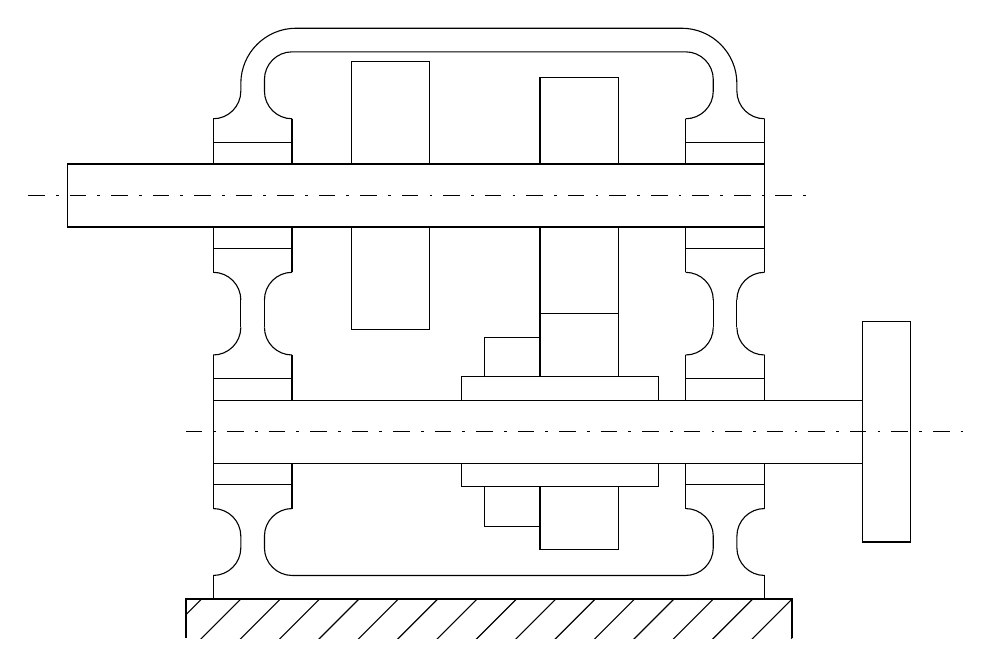
\begin{tikzpicture}

\newcommand{\flansch}[4]{
	\draw[#3,rounded corners=10]
	(#1,#2)--++(0,0.35*#4)--($(#1,#2)+(0.35*#4,0.35*#4)$);
	\draw[#3] ($(#1,#2)+(0.5*#4,0.35*#4)-(#4*0.15,0)$)--++
	(0,0.3*#4)--++(-#4,0)--++(0,-0.3*#4);
	\draw[#3,rounded corners=10]
	($(#1,#2)-(#4*0.3,0)$)--++(0,0.35*#4)--($(#1,#2)+(-#4*0.65,0.35*#4)$);
	
	\draw[#3]($(#1,#2)+(-#4*0.65,2.3*#4)$)
	--++(0,-0.3*#4)--++(#4,0)--++(0,0.3*#4);
	\draw[#3,rounded corners=10]
	($(#1,#2)+(-#4*0.65,2.3*#4)$)--++(0.35*#4,0)--++(0,0.35*#4);
	\draw[#3,rounded corners=10]
	($(#1,#2)+(#4*0.35,2.3*#4)$)--++(-0.35*#4,0)--++(0,0.35*#4);
};
%	MASSE:
%	gesamte Hoehe: 2.65 * #4
%	Breite ansatz: 0.3 * #4
%	Breite am Kopf: #4
%	Wellendurchmesser: 2 * #4
% 	Position von #1 und #2 : rechtes unteres Ende
%	#3 Optionen der Zeichnung


%%% GEHAEUSE
\flansch{0}{1}{}{1};
\flansch{0}{4}{}{1};
\flansch{6}{1}{}{1};
\flansch{6}{4}{}{1};

\draw (0,3.65)--(0,4);
\draw (-0.3,3.65)--(-0.3,4);
\draw (6,3.65)--(6,4);
\draw (5.7,3.65)--(5.7,4);

\draw[rounded corners=10] (0,1)--(0,0.5)--(5.7,0.5)--(5.7,1);
\draw[rounded corners=10] (-0.3,1)--(-0.3,0.5)--(-0.65,0.5);
\draw[rounded corners=10] (6.35,0.5)--(6,0.5)--(6,1);
\draw (-0.65,0.5)--(-0.65,0.2)--(6.35,0.2)--(6.35,0.5);

\draw[rounded corners=20] (6,6.65)--++(0,0.8)--++(-6.3,0)--++(0,-0.8);
\draw[rounded corners=10] (5.7,6.65)--++(0,0.5)--++(-5.7,0)--++(0,-0.5);


%%%INNENLEBEN

%LAGER
\draw[] (0.35,1.65) rectangle (-.65,3);
\draw[] (0.35,4.65) rectangle (-.65,6);
\draw[] (6.35,4.65) rectangle (5.35,6);
\draw[] (6.35,1.65) rectangle (5.35,3);

%WELLENAUFSATZ
\draw ($(2.8,2.325)+(0,-1.2)$) rectangle($(2.8,2.325)+(0.7,1.2)$);
\draw[fill=white] ($(3.5,2.325)+(0,-1.5)$) rectangle($(3.5,2.325)+(1,1.5)$);
\draw[fill=white] ($(2.5,2.325)+(0,-0.7)$) rectangle(5,3.025);

\draw[fill=white] ($(3.5,5.325)+(0,-1.5)$) rectangle($(3.5,5.325)+(1,1.5)$);
\draw[fill=white] ($(1.1,5.325)+(0,-1.7)$) rectangle($(1.1,5.325)+(1,1.7)$);

%WELLEN
\draw[fill=white] ($(-2.5,5.325)+(0,-0.4)$) rectangle($(-2.5,5.325)+(8.85,0.4)$);

\draw[fill=white] ($(-0.65,2.325)+(0,-0.4)$) rectangle($(-0.65,2.325)+(8.85,0.4)$);

%AUSSEN
\draw[fill=white] ($(8.2,2.325)+(0,-1.4)$) rectangle($(8.2,2.325)+(-0.6,1.4)$);

%%%MITTELLINIEN
\draw[dash pattern=on 6pt off 4pt on 1pt off 4pt] ($(-1,1)+(0,2.65/2)$)--++(10,0);
\draw[dash pattern=on 6pt off 4pt on 1pt off 4pt] ($(-3,4)+(0,2.65/2)$)--++(10,0);


%BODEN
\begin{scope}
\clip (-1,0.2) rectangle (6.7,-0.3);
\foreach \x in {-3,-2.5,...,7}
\draw (\x,-1)--(\x+2,1);
\end{scope}
\draw[thick] (-1,-0.3)--(-1,0.2)--(6.7,0.2)--(6.7,-0.3);

\end{tikzpicture}
\par\end{centering}
\caption{}
\end{figure}

hallo


\end{document}